

\section{Learning low-level vision}

Orientation is an important visual cue for many purposes, such as
object segmentation, recognition, and tracking.  It is associated with
neighborhoods rather than individual points in an image, and so is
inherently scale dependent.  At very fine scales, relatively few
pixels are available from which to judge orientation.
Lines and edges at such scales are extremely pixelated and
rough.
%
Orientation filters derived from analytic considerations, with
parameters chosen assuming smooth, ideal straight lines or edges (for
example, \cite{chen00orientation}) are more suited to larger
neighborhoods with more redundant information.
For fine scales, an empirical approach seems more promising, particularly
given that when the number of pixels involved is low, it is practical
to sample the space of all possible appearances of these pixels 
quite densely.

The data collected during poking allows us to explore how edges truly
look in ``natural'' images, by simply building up a catalog of edge
fragments seen around the boundaries of objects.  Of course, such a
catalog is only practical at small scales.  We worked with $4\times 4$
pixel windows, a size is chosen to be large enough to be interesting,
but small enough for the complete range of possible appearances to be
easily visualized.  Even at this scale, manual data collection and
labelling would be extremely tedious, so it is definitely advantageous
to have a robotic system to automatically compile and label a database
of the appearance of oriented features.
%
%, as shown in Figure~\ref{fig:separate-simple}.  
%Details of this procedure are given in
%Section~\ref{sect:experiment}.
These features were extracted by sampling image patches
along object boundaries, which were in turn determined 
using active segmentation~\cite{fitzpatrick03first}.
The resulting catalog of edge appearances proved remarkably
diverse, although the most frequent appearances were indeed
the ``ideal'' straight, noise-free edge.

%Figures~\ref{fig:lines-all} and ~\ref{fig:seen-selected}.
Figure~\ref{fig:seen-selected}.

\begin{figure}[bt]
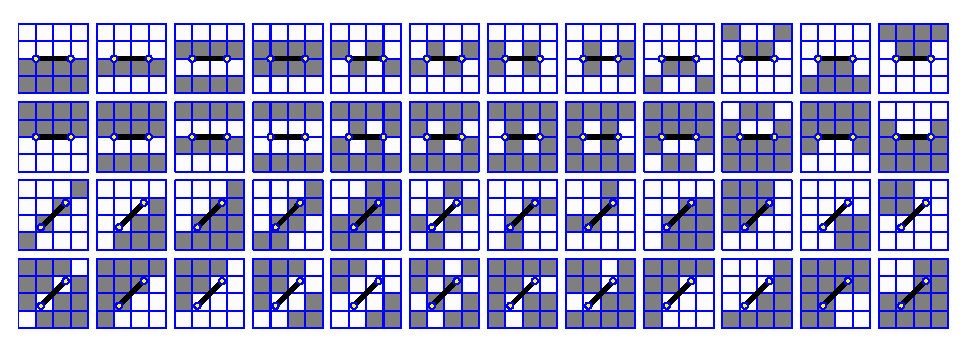
\includegraphics[width=\columnwidth]{seen-selected}
\caption
{
\label{fig:seen-selected}
%
Edges have diverse appearances.  This figure shows 
the orientations assigned to a test suite
prepared by hand.  Each $4\times 4$ grid is a single test
edge patch, and the dark line centered in the grid is the orientation
that patch was observed to have in the training data.
The oriented features represented
include edges, thin lines, thick lines, zig-zags, corners
etc.  It is difficult to imagine a set of conventional
filters that could respond correctly to the full range of 
features seen here~-- all of which appeared multiple
times in object boundaries in real images.
%
}
\end{figure}

\ifnote
\begin{figure}[tb]
\begin{center}
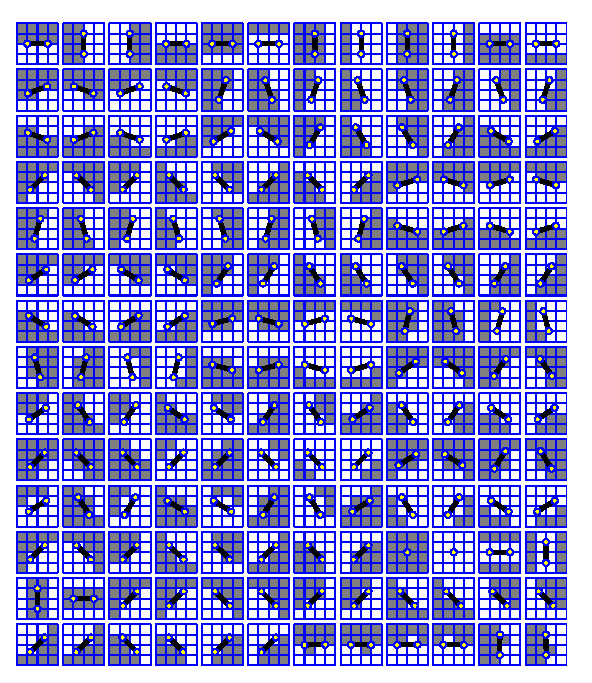
\includegraphics[width=\columnwidth]{seen-all}
\caption{
\label{fig:lines-all}
%
The most frequently observed edge appearances.  All patches
observed are replicated for all $90^{\circ}$ rotations, mirror flips,
and inversion of foreground/background.
%
The most frequent (top) are simple straight edges.
%
The line in the center of
each patch shows the orientation associated with that patch.  
%
After the straight edges, the completely empty patch
is common (produced in saturated regions), 
followed by a tube-like feature (third-last row)
where the boundary is visually distinct to either side of
the edge.
This is followed corner-like features and
many thousands of variations on the themes already seen.  
%
}
\end{center}
\end{figure}
\fi
